%! TEX root = main.tex

\graphicspath{{00_Images/11_chapter/}}

\chapter{Automatic Gain Control Circuits}
\label{ch:agc}

\section{General Concept and Block Diagram}
\label{sc:111}

An automatic gain control circuit adapts the gain of a stage dynamically, in response to the amplitude of the signal it is processing, rather than keeping a fixed amplification.
The purpose is to manage the dynamic range of the audio: to compress or limit the loud passages that exceed a chosen level, and to expand or gate the quiet passages that fall below it, so that the program material fits within the operating window of the following equipment.
The element that makes this possible is the voltage controlled amplifier introduced in section \ref{sc:644}, whose gain is steered by a control voltage \(V_c\):
\[
v_{out} = G(V_c) v_{in}
\]

\begin{figure}[!htb]
    \centering
    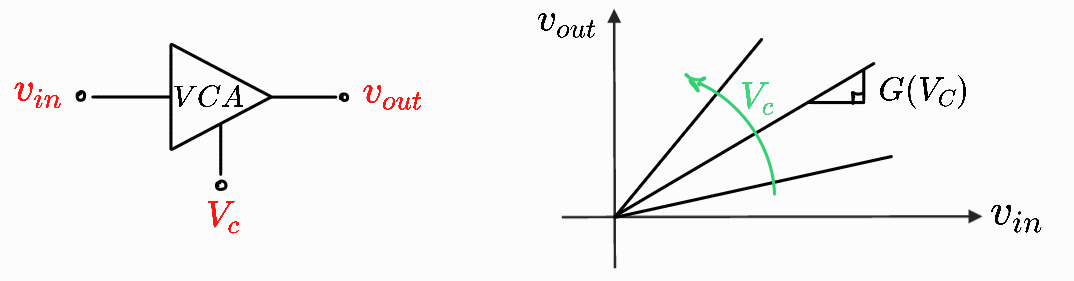
\includegraphics[width=0.70\textwidth]{VCA.png}
    \caption{The voltage controlled amplifier and its control characteristic: the gain \(G\) is a function of the control voltage \(V_c\)}
    \label{fig:vca}
\end{figure}

The control voltage cannot be derived from the instantaneous signal, which swings rapidly through zero, but from a measure of its average level.
This requires the root-mean-square value of the signal, computed by a chain of three operations: a multiplier that squares the signal, an integrator that averages the square over a short window, and a square-root operator that recovers the amplitude.

\begin{figure}[!htb]
    \centering
    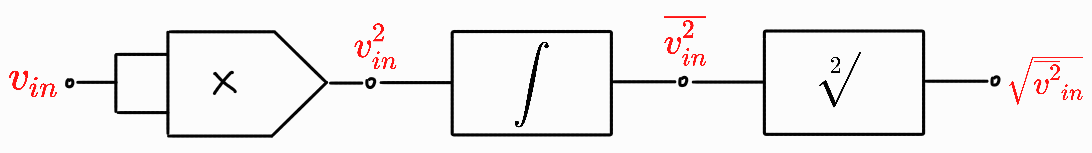
\includegraphics[width=0.70\textwidth]{RMS_Pipeline.png}
    \caption{Root-mean-square detection pipeline: the signal is squared, time-averaged by an integrator, and then passed through a square-root operator}
    \label{fig:rmsPipeline}
\end{figure}

The multiplier forms \(v_{out} = v_a v_b\) and, with both inputs equal, the square \(v_{in}^2\); the integrator computes the running average
\[
\overline{v} = \frac{1}{T}\int_T v(\tau) d\tau \quad \Rightarrow \quad v_{out}(t) = -\frac{1}{RC}\int v_{in}(t) dt
\]
in inverting operational amplifier form; and the square-root operator, obtained by placing a squaring multiplier in the feedback path of an inverting stage, returns \(v_{out} = \sqrt{-(R_2/R_1) v_{in}}\), valid for a negative input as guaranteed by the preceding inverting stage.
For a sinusoidal input the result is the familiar \(v_{RMS} = v_{peak}/\sqrt{2}\).
In a practical design this whole chain is realized by a dedicated root-mean-square-to-DC converter integrated circuit, such as the AD8436, which delivers a clean DC voltage proportional to the signal level.
The complete automatic gain control loop is therefore a sidechain wrapped around the signal path, as in figure \ref{fig:agcBlock}.
The signal is tapped after the voltage controlled amplifier, its level is measured by the root-mean-square detector and smoothed by a filter, and the resulting DC level is compared against a threshold voltage \(V_{TH}\) by a comparator.
The comparator output becomes the control voltage that sets the gain, so that whenever the signal level rises above the threshold the gain is reduced, and the loop closes:
\[
v_{in,RMS} > V_{TH} \quad \Rightarrow \quad \text{the gain is lowered and the signal is attenuated}
\]

\begin{figure}[!htb]
    \centering
    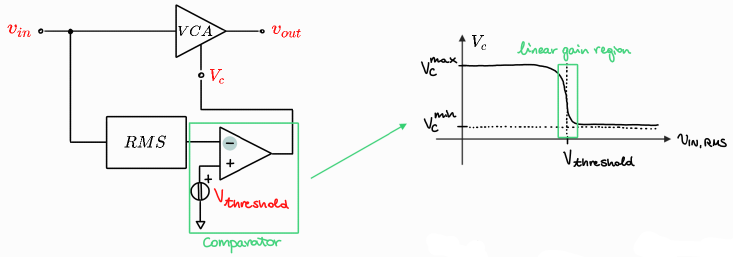
\includegraphics[width=0.70\textwidth]{AGC_Circuit.png}
    \caption{Automatic gain control as a sidechain loop: the signal level is detected, compared with the threshold \(V_{TH}\), and fed back as the control voltage of the voltage controlled amplifier}
    \label{fig:agcBlock}
\end{figure}

\section{Compressor and Limiter}
\label{sc:112}

A compressor reduces the dynamic range of the signals whose level exceeds the threshold \(V_{TH}\), bringing the loud passages closer to the quiet ones.
Its action is described by the curve of output level against input level, both taken as root-mean-square values: below the threshold the slope is unity, so the signal passes unaltered, while above the threshold the slope is reduced.

\begin{figure}[!htb]
    \centering
    \subfloat[Output versus input level: unity slope below threshold, reduced slope above]{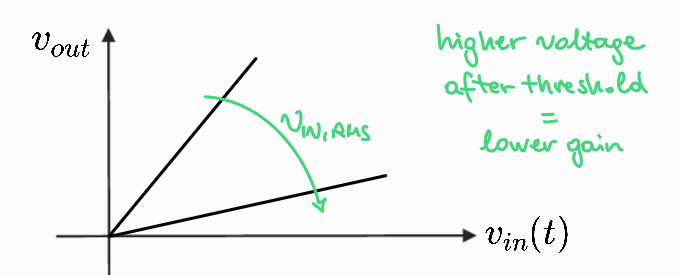
\includegraphics[height=0.13\textheight]{linear_scale.png}}
    \hfill
    \subfloat[Effect on a growing signal: the compressed output stays below the uncompressed one above threshold]{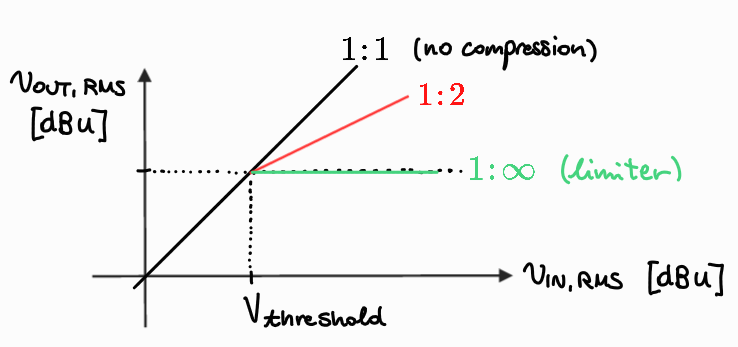
\includegraphics[height=0.13\textheight]{limiter_comparison.png}}
    \caption{The compression characteristic and its effect on the signal envelope}
    \label{fig:compressionCharacteristic}
\end{figure}

The degree of compression is quantified by the compression ratio.
A ratio of \(k\colon 1\) means that an increase of \(k\) decibels at the input produces an increase of only one decibel at the output, so the larger the ratio the flatter the response above threshold, common values being \(2\colon 1\) and \(4\colon 1\).
The transition at the threshold can be abrupt or gradual: a hard knee switches sharply into compression exactly at the threshold, while a soft knee blends the slope change over a range around it, for a more transparent action.

\begin{figure}[!htb]
    \centering
    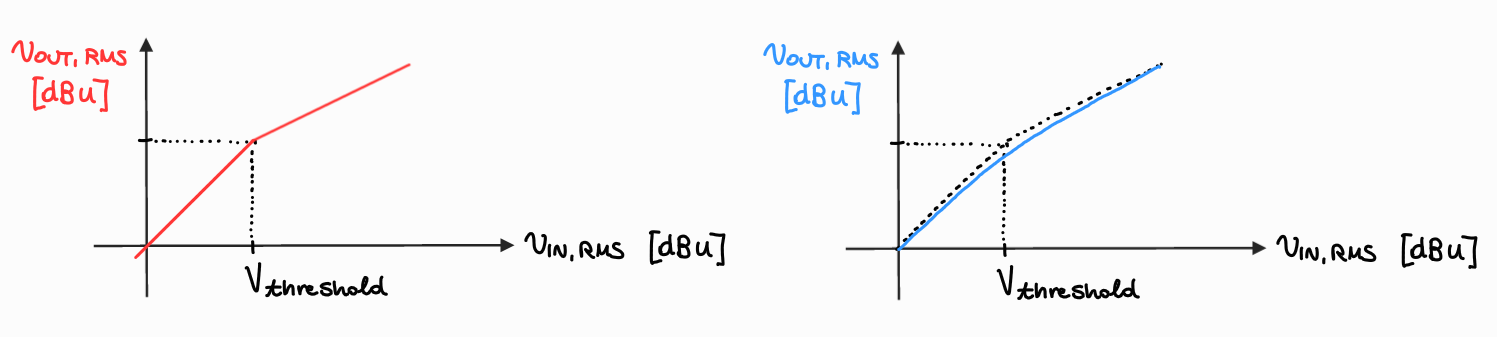
\includegraphics[width=0.70\textwidth]{Hard_Knee_Soft_Knee.png}
    \caption{Hard knee, with an abrupt onset at the threshold, against soft knee, with a gradual onset around it}
    \label{fig:knee}
\end{figure}

A limiter is the extreme case of a compressor, with a compression ratio of \(\infty\colon 1\), so that the output level can never rise above the threshold no matter how large the input becomes.
It is essential to distinguish a limiter from a clipper, because the two prevent the same overshoot in fundamentally different ways.
A limiter acts through gain control: it reduces the gain \(G\) so that the waveform is scaled down but kept intact, preserving its shape and introducing no new harmonic content.
A clipper, by contrast, truncates the waveform above the threshold with a hard cut, exactly the hard-clipping mechanism analyzed for the MXR Distortion+ in section \ref{sc:34}, and this discontinuity generates harmonic distortion.
A limiter therefore controls level transparently, whereas a clipper controls level at the cost of distortion.

\begin{figure}[!htb]
    \centering
    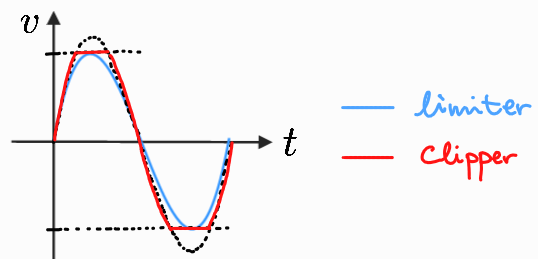
\includegraphics[width=0.70\textwidth]{Limiter_vs_Clipper.png}
    \caption{Limiter against clipper: the limiter scales the waveform while preserving its shape, the clipper truncates it}
    \label{fig:limiterClipper}
\end{figure}

Because the level detector relies on an averaging integrator, the gain change is not instantaneous but governed by two time constants.
The attack time is how quickly the system lowers the gain when the input amplitude suddenly increases, and the release time is how long it takes to restore the gain back toward unity after the input subsides.
The complete gain law is thus a function of the signal history together with the threshold and the ratio:
\[
G(t) = f\big(v_{in}(t), V_{TH}, t_{attack}, t_{release}, k\big)
\]
The choice of these times shapes the audible behavior of the processor: a fast attack catches transients tightly, while a slow release avoids audible pumping of the background level.

\begin{figure}[!htb]
    \centering
    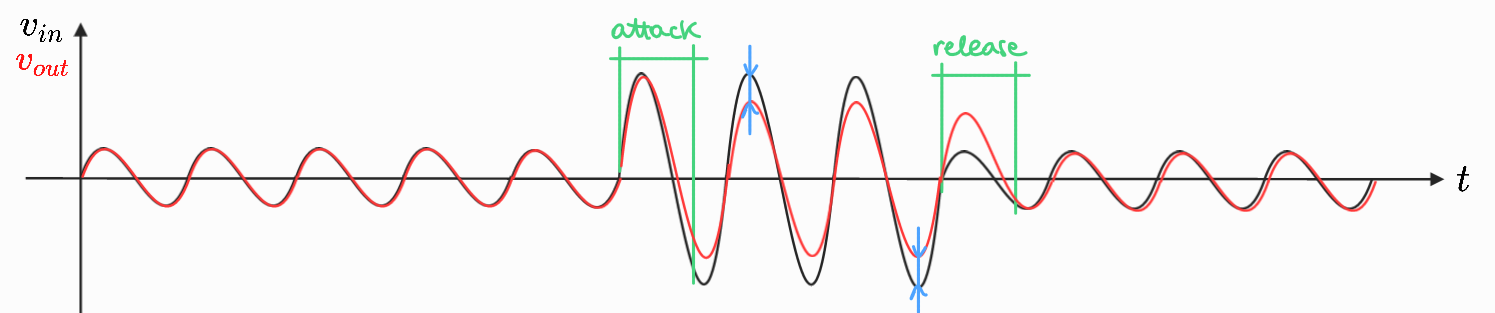
\includegraphics[width=0.75\textwidth]{Limiter.png}
    \caption{Time evolution of the gain reduction, showing the attack phase as the level crosses the threshold and the release phase as it returns}
    \label{fig:attackRelease}
\end{figure}

\section{Gate and Expander}
\label{sc:113}

Where the compressor and limiter act on signals above the threshold, the expander and the gate act on signals below it, controlling the quiet end of the dynamic range.
The circuit is the same sidechain as before, with the comparator inputs exchanged, the detected level applied to the inverting input and the threshold to the non-inverting input, so that the loop now reacts when the signal falls below \(V_{TH}\).

\begin{figure}[!htb]
    \centering
    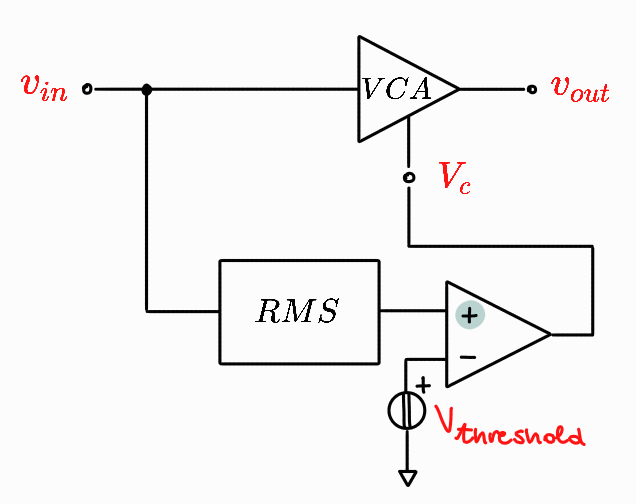
\includegraphics[width=0.40\textwidth]{Gate_Expander_Circuit.png}
    \caption{Gate and expander sidechain: the comparator inputs are swapped with respect to the compressor, so the gain is reduced for signals below the threshold}
    \label{fig:gateExpanderCircuit}
\end{figure}

An expander attenuates the signals that lie below the threshold by a controlled amount, set by an expansion ratio such as \(1\colon 2\), pushing the weak passages further down while leaving the loud ones untouched.
The effect is the opposite of compression: the difference between the quiet and the loud parts of the program is increased, so the dynamic range is enlarged rather than reduced.
A gate, or noise gate, is the extreme expander that does not merely attenuate but strongly suppresses, or switches off, any signal below the threshold.
Its typical use is to remove the background noise studied in chapter \ref{ch:noise} during the pauses of a performance, since the residual hiss and hum sit below the threshold and are silenced when no wanted signal is present.

\begin{figure}[!htb]
    \centering
    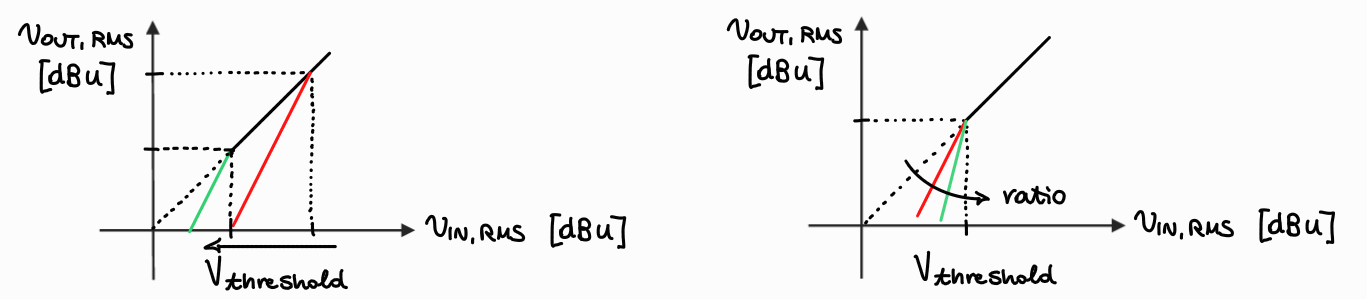
\includegraphics[width=0.70\textwidth]{Gate_vs_Expander.png}
    \caption{Characteristics of the gate, which cuts the signal below the threshold, and of the expander, which attenuates it gradually}
    \label{fig:gateVsExpander}
\end{figure}

The direction of the expansion can also be reversed.
A downward expander lowers the level of the signals below the threshold, the common case described above, whereas an upward expander raises the level of the signals above the threshold, widening the dynamics from the top instead.

\begin{figure}[!htb]
    \centering
    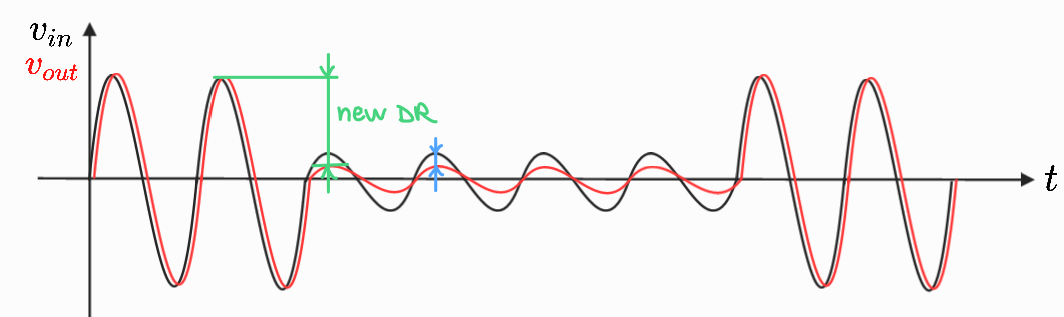
\includegraphics[width=0.70\textwidth]{Expander_Dynamic_Control.png}
    \caption{Downward and upward expansion as two ways of enlarging the dynamic range}
    \label{fig:expanderDynamics}
\end{figure}

Two refinements of the same principle are widely used in practice.
A de-esser is a compressor that acts only on a restricted frequency band, used to tame the sibilant consonants of a vocal track without affecting the rest of the spectrum.
A sidechain compressor takes its threshold control from an external signal rather than from the processed one, the classic application being the automatic lowering of background music whenever a voice is detected, a technique routinely employed in broadcasting.
